\subsection{DOM Engine}

KHTML/WebKit (KDE, Apple), JavaScriptCore or V8 (Google);
The Gecko engine (Mozilla Corporation) and it's JavaScript implementation Spidermonkey;
We briefly checked on Presto (Opera) and Trident (Microsoft), but discarded them due to their proprietary nature.

\subsubsection{Firefox AddOn}

To avoid interference with other AddOns and existing configuration, we suggest creating a new browser profile for use with the AddOn.
For easy use, Firefox' proxy configuration is automatically pointed to a preconfigured host and the user is directed to a special landing page upon successful installation.
Furthermore, the installation binary is digitaly signed, so the user does not have to go through various exception dialogs.


Once installed, the functionality of the AddOn is available via a broom icon in the status bar.
While it offers lots of functions around annotation and corpus selection, it's core feature is simple:
In highlight mode (the broom turns fuchsia) mouse hovering over the page will highlight the text blocks below the cursor.
The block can then be annotated using the context-menu or a keyboard short-cut, which will change its color to the one corresponding to the annotation class.
Figure \ref{f:tut0} shows a fully annotated page and the context-menu.

\begin{figure}
\jss{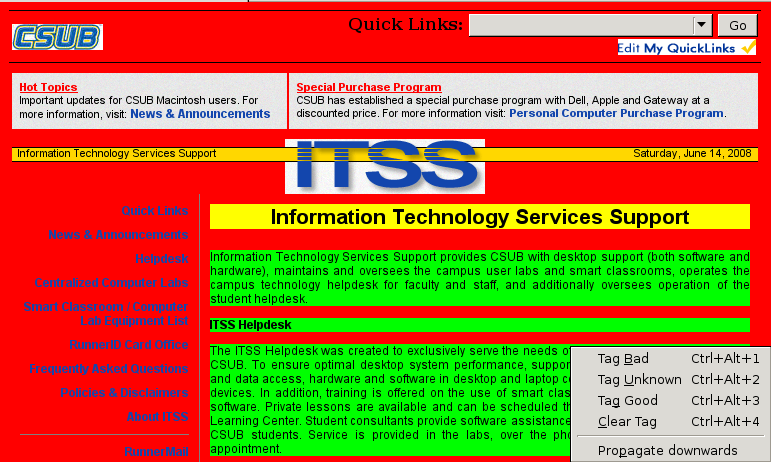
\includegraphics[width=0.5\textwidth]{tut0}}
	{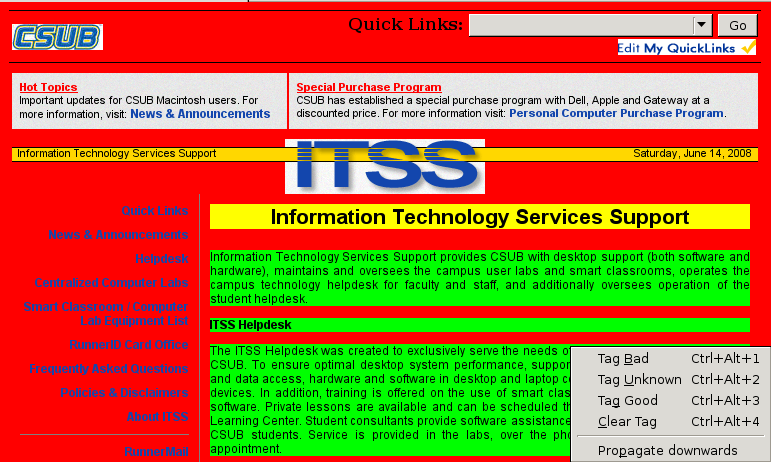
\includegraphics[width=\textwidth]{tut0}}
\caption{\label{f:tut0}Web pages can be annotated with the \KrdWrd Firefox AddOn by hovering over the text by mouse and setting class labels by keyboard short-cut or pop-up menu}
\end{figure}


\subsubsection{XUL Application \label{app}}

The XUL application (or \textit{app} for short) 
Dumper, Grabber, Crawler

% ens said: if you like:
% \cite{NajorkHeydon2001,ShkapenyukSuel2002}

\subsection{Storage and Control}

database and web server. 
html hosted on own server, with baseurl; all other data through proxy; initially populated by the grabber described in \ref{app}.
user annotations list of tags, one entry for every text node, in dom tree order;


\subsubsection{Web Server}

small Python CGI scripts;
provides per-corpora submission list,
controls serving of random corpus pages;
tutorial mode: visual diff after submit;
ssl connections only;

\begin{figure}
\jss{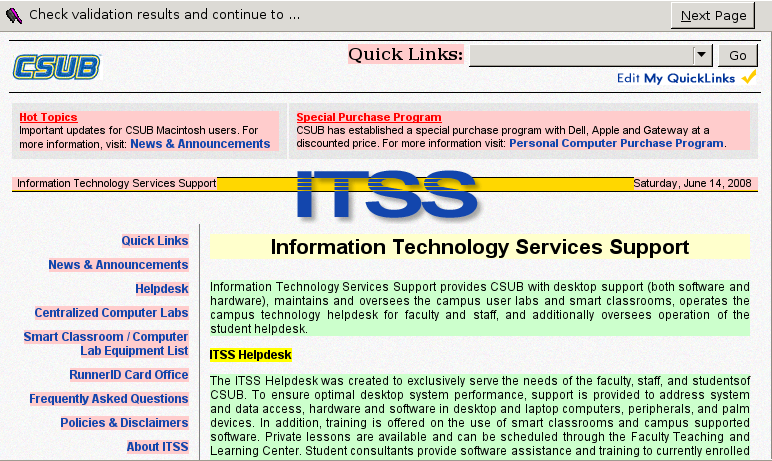
\includegraphics[width=0.5\textwidth]{tut1}}
	{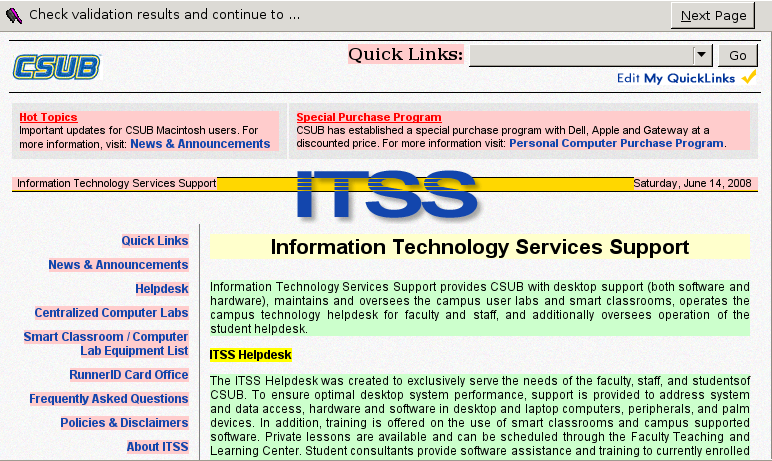
\includegraphics[width=\textwidth]{tut1}}
\caption{\label{f:tut1}During the tutorial, a Visual Diff between the user's submission and the sample data is presented right after submission.
	Here, the annotation from \ref{f:tut0} was wrong in tagging the sub-heading ``ITSS Helpdesk'': the correct annotation (\textit{yellow}) is highlighted in the feedback.}
\end{figure}

\subsubsection{Database}

Raw HTML in sqlite3;
user submissions are anonymized, but trackable by id;

\subsubsection{Proxy}

\begin{figure}
\jss{
\includegraphics[width=0.5\textwidth]{add}}
	{
\includegraphics[width=\textwidth]{add}}
\caption{IFrames with dynamic URLs which usually come from advertisements are blocked as a nice side-effect of the Proxy setup}
\end{figure}

\subsection{Feature Extractors}

app produces input files for pipelines, dumped in the filesystem, per-page with one line per dom text node;
integrated dom feature extraction;
integrated screen grab;

\subsubsection{Text}

Dumped raw text, leading and trailing whitespace removed, UTF-8.

\subsubsection{Meta Visual}

Use data from living DOM Tree in XUL App.

\subsubsection{Visual}

Screenshot and use JAMF as seen in \cite{Steger08}
\footnote{This Extractor requires at least XULRunner Version 1.9.2 (corresponding to Firefox Version 3.5) which is still in beta at the time of this writing}

\subsection{Machine Learner}

Generic input vectors and classes from extractors

\subsection{\label{sec:limitations}Highlights and Limitations}

html, utf, js, iframes
